\documentclass[a4paper,10pt]{article}
\usepackage[a4paper, hmargin={2cm,2cm}, vmargin={1.5cm,1.5cm}]{geometry}
\usepackage{amsmath}
\usepackage{amsthm}
\usepackage{amsfonts}
\usepackage{color}
\usepackage{graphicx}
\usepackage{listings}

\newcommand{\R}{\mathbb{R}}

\begin{document}

\section{Incompressible Navier Stokes Equation}

\subsection{Problem}
We want to find \[(u,p) : \Omega \times (0,T) \rightarrow \R^d \times \R\] where $ u $ is unknown velocity and $ p $ is unknown pressure such that
\begin{equation}\label{Navier-Stokes}
\begin{cases}
\dfrac{\partial u}{\partial t} + (u \cdot \nabla) u - \nu \bigtriangleup u + \nabla p = f & \text{ in } \Omega \times (0,T)\\
\nabla \cdot u = 0 & \text{ in } \Omega \times (0,T)\\
u = 0 & \text{ on } \partial \Omega \times (0,T)\\
u = u^0 & \text{ in } \Omega \text{, at } t=0
\end{cases}
\end{equation}
where $ f : \Omega \times (0,T) \rightarrow \R^d $ and $ u^0 : \Omega \rightarrow \R^d $ are given functions, $ \nu > 0 $ is a viscosity.

\subsection{Weak Form}
The weak formulation for equation (\ref{Navier-Stokes}) is shown below. We want to find $ \{ (u,p)(t) \in V \times Q ; t \in (0.T) \} $ such that for $ t \in (0,T) $
\begin{equation} \label{NS_Weak}
\begin{cases}
\big( \dfrac{\partial u}{\partial t} + (u \cdot \nabla)u,v \big) + a(u,v) + b(v,p) + b(u,q) = (f,v) & ,\forall(v,q)\in V\times Q \\ u=u^{0} & , t=0
\end{cases}
\end{equation}
where
\begin{eqnarray}\nonumber
a(u,v) &=& \nu \int_{\Omega} \nabla u : \nabla v \ dx \\ \nonumber
b(v,q) &=& - \int_{\Omega} (\nabla \cdot v) q \ dx \\ \nonumber
V &=& H_{0}^{1}(\Omega, \R^d) = H_{0}^{1}(\Omega)^d \\ \nonumber
Q &=& \{ q\in L^2(\Omega) ; \int_{\Omega} q \ dx=0 \}.
\end{eqnarray}

\subsection{Error estimate}
To estimate the error in 2D, we use $ L_{2} $-norm
\begin{eqnarray}\nonumber
E(h,dt) &=& \| u_{h}^{n}-u^{n} \|_{L^\infty(L^2)} \\ \nonumber
&=& max \ \| u_{h}^{n}-u^{n} \|_{L^2(\Omega)}^{2} \\ \nonumber
&=& max \ \{ \| u_{h_{1}}^{n}-u_{1}^{n} \|_{L^2(\Omega)}^{2} + \| u_{h_{2}}^{n}-u_{2}^{n} \|_{L^2(\Omega)}^{2} \}^{1/2} \\ \nonumber
&=& max \ \{ \int_{\Omega} (u_{h_{1}}^{n}-u_{1}^{n})^2 \ dx + \int_{\Omega} (u_{h_{2}}^{n}-u_{2}^{n})^2 \ dx \}^{1/2}
\end{eqnarray}
To estimate the error in 3D, we use
\begin{eqnarray}\nonumber
E(h,dt) &=& \| u_{h}^{n}-u^{n} \|_{L^\infty(L^2)} \\ \nonumber
&=& max \ \| u_{h}^{n}-u^{n} \| \\ \nonumber
&=& max \ \{ \| u_{h_{1}}^{n}-u_{1}^{n} \|_{L^2(\Omega)}^{2} + \| u_{h_{2}}^{n}-u_{2}^{n} \|_{L^2(\Omega)}^{2} + \| u_{h_{3}}^{n}-u_{3}^{n} \|_{L^2(\Omega)}^{2} \}^{1/2} \\ \nonumber
&=& max \ \{ \int_{\Omega} (u_{h_{1}}^{n}-u_{1}^{n})^2 \ dx + \int_{\Omega} (u_{h_{2}}^{n}-u_{2}^{n})^2 \ dx +  \int_{\Omega} (u_{h_{3}}^{n}-u_{3}^{n})^2 \ dx \}^{1/2}
\end{eqnarray}

To estimate the error, we also use $ H $-norm
\[ E(h,dt) = \| u_{h}^{n}-u^{n} \|_{L^\infty(H^{1})} = max \sqrt{\| u_{h_{1}}^{n}-u_{1}^{n} \|_{L^2(\Omega)}^{2} + \| \nabla (u_{h_{1}}^{n}-u_{1}^{n}) \|_{L^2(\Omega)}^{2}} \]

\newpage
\subsection{ 2D Simulation}
Below, is the exact solution to check if the program for 2D is working.
\begin{eqnarray} \nonumber
u &=& (u_{1},u_{2})\\ \nonumber
u_{1} &=& -cos(x_{1}) sin(x_{2}) e^{-4t} \\\nonumber
u_{2} &=& -sin(x_{1}) cos(x_{2}) e^{-4t} \\\nonumber
p &=& \dfrac{1}{4} (cos(2x_{1}) + cos(2x_{2})) e^{-4t}
\end{eqnarray}
such that equation (\ref{Navier-Stokes}) is satisfied with $ f = (f_{1},f_{2}) $. \\With $ f_{1} = -e^{-4t}sin(2x_{1}) $ and $ f_{2} = -e^{-4t} sin(2x_{2}) $.

with the error estimate :
\begin{figure}[h!]
	\centering
	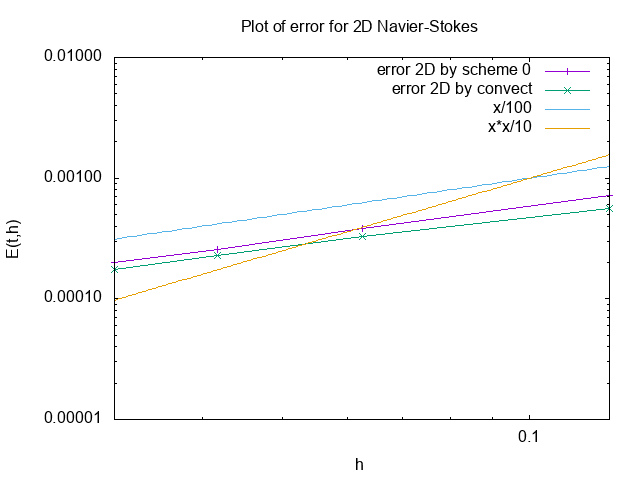
\includegraphics[width=0.7\linewidth]{NS_2D/error_NS_2D}
	\caption{}
	\label{fig:errorns2d}
\end{figure}

As we can see, the error using convect is slightly better than scheme $ 0 $. By the graphic, we have $ O(h) $.

\newpage
Below is the FreeFEM++ code used to solve the problem above with the discritization of time using scheme $ 0 $ :
\begin{lstlisting}
load "iovtk"

// Variable declaration
real nu = 1.0;
real Lx = 1.0;
real Ly = 1.0;
real error;
real errormax = 0.;
real t=0;
func exactu = -cos(x)*sin(y)*exp(-2*t);
func exactv = sin(x)*cos(y)*exp(-2*t);
func f1 = -exp(-4*t)*sin(2*x);
func f2 = -exp(-4*t)*sin(2*y);

//  Set the border
border c1 (t=0,1)    {x=t*Lx; y=0;}
border c2 (t=0,1)    {x=Lx; y=t*Ly;}
border c3 (t=1,0)    {x=t*Lx; y=Ly;}
border c4 (t=1,0)    {x=0; y=t*Ly;}

ofstream ff("error2D.txt");
ofstream pp("p.txt");

//iteration for each mesh devider
for(int n=32; n>=8; n=n-8 )
{
real dt = 1./n; //take dt=h

//  Create the mesh
mesh Th = buildmesh ( c1(n)+c2(n)+c3(n)+c4(n) );
plot ( Th, ps = "NS_2D_mesh.ps" );

//  Define the finite element spaces for velocity and pressure
fespace Uh(Th, P2);
fespace Vh(Th, P1);
Uh u, v, uh, vh, uold, vold;
Vh p, ph;

//  Set up the Navier−Stokes equationss
uold = -cos(x)*sin(y) ;
vold = sin(x)*cos(y) ;

problem navierstokes ( [u,v,p], [uh,vh,ph] ) =
int2d(Th) (u*uh/dt) - int2d(Th) (uold*uh/dt)
+ int2d(Th) (v*vh/dt) - int2d(Th) (vold*vh/dt)
+ int2d(Th) (uold*dx(u)*uh + vold*dy(u)*uh)
+ int2d(Th) (uold*dx(v)*vh + vold*dy(v)*vh)
+ int2d(Th) (nu*dx(u)*dx(uh) + nu*dy(u)*dy(uh) )
+ int2d(Th) (nu*dx(v)*dx(vh) + nu*dy(v)*dy(vh) )
- int2d(Th) (p*dx(uh)+ p*dy(vh))
- int2d(Th) (dx(u)*ph + dy(v)*ph)
- int2d(Th) (f1*uh)
- int2d(Th) (f2*vh)
+ on ( c1, c2, c3, c4, u=exactu, v=exactv);

for ( int it = 1; it <= n; it++ )
{
t=it*dt;
navierstokes;
error = sqrt( int2d(Th)((u-exactu)*(u-exactu)) + int2d(Th)((v-exactv)*(v-exactv)) );
if (error > errormax) errormax = error ;
//cout << "error at " << t << "is " << error << "\n" ;
if(n==32){
plot ( Th, [u,v], nbiso = 60, fill = 0, value = 1, wait = 0, ps = "NS_2D_"+n+"_"+it+".ps" );
savevtk("NS_2D_plot"+n+"_"+it+".vtk",Th,[u,v],p,dataname="NS");
plot (p, nbiso=60, fill =0, value =1, wait =0, ps = "NS_2D-C-p_"+n+"_"+it+".ps" );
pp << t << "\t" << p << "\n" ;
}
uold = u;
vold = v;
}
ff << dt << "\t" << errormax << "\n" ;
cout << ">>>>>MESH>>>>> " << n << " executed \n" ;
errormax = 0;
}
//  Terminate.
//
cout << "\n";
cout << "NAVIERSTOKES_2D:\n";
cout << "Normal end of execution.\n";

\end{lstlisting}

\newpage
We also try to use convect function instead, the code is :
\begin{lstlisting}
load "iovtk"

// Variable declaration
real nu = 1.0;
real Lx = 1.0;
real Ly = 1.0;
real error;
real errormax = 0.;
real t=0;
func exactu = -cos(x)*sin(y)*exp(-2*t);
func exactv = sin(x)*cos(y)*exp(-2*t);
func f1 = -exp(-4*t)*sin(2*x);
func f2 = -exp(-4*t)*sin(2*y);


//  Set the border
border c1 (t=0,1)    {x=t*Lx; y=0;}
border c2 (t=0,1)    {x=Lx; y=t*Ly;}
border c3 (t=1,0)    {x=t*Lx; y=Ly;}
border c4 (t=1,0)    {x=0; y=t*Ly;}

ofstream ff("error2D-C.txt");
ofstream pp("p-C.txt");

//iteration for each mesh devider
for(int n=32; n>=8; n=n-8 )
{
real dt = 1./n; //take dt=h

//  Create the mesh
mesh Th = buildmesh ( c1(n)+c2(n)+c3(n)+c4(n) );
plot ( Th, ps = "NS_2D-C_mesh.ps" );

//  Define the finite element spaces for velocity and pressure
fespace Uh(Th, P2);
fespace Vh(Th, P1);
Uh u, v, uh, vh, uold, vold;
Vh p, ph;

//  Set up the Navier−Stokes equationss
uold = -cos(x)*sin(y) ;
vold = sin(x)*cos(y) ;

problem navierstokes ( [u,v,p], [uh,vh,ph] ) =
int2d(Th) (u*uh/dt) - int2d(Th) (convect([uold,vold],(-dt),uold)*uh/dt)
+ int2d(Th) (v*vh/dt) - int2d(Th) (convect([uold,vold],(-dt),vold)*vh/dt)
+ int2d(Th) (nu*dx(u)*dx(uh) + nu*dy(u)*dy(uh) )
+ int2d(Th) (nu*dx(v)*dx(vh) + nu*dy(v)*dy(vh) )
- int2d(Th) (p*dx(uh)+ p*dy(vh))
- int2d(Th) (dx(u)*ph + dy(v)*ph)
- int2d(Th) (f1*uh)
- int2d(Th) (f2*vh)
+ on ( c1, c2, c3, c4, u=exactu, v=exactv);

for ( int it = 1; it <= n; it++ )
{
t=it*dt;
navierstokes;
error = sqrt( int2d(Th)((u-exactu)*(u-exactu)) + int2d(Th)((v-exactv)*(v-exactv)) );
if (error > errormax) errormax = error ;
//cout << "error at " << t << "is " << error << "\n" ;
if(n==32){
plot ( Th, [u,v], nbiso = 60, fill = 0, value = 1, wait = 0, ps = "NS_2D-C_"+n+"_"+it+".ps" );
savevtk("NS_2D-C_plot"+n+"_"+it+".vtk",Th,[u,v],p,dataname="NS");
plot (p, nbiso=60, fill =0, value =1, wait =0, ps = "NS_2D-C-p_"+n+"_"+it+".ps" );
pp << t << "\t" << p << "\n" ;
}
uold = u;
vold = v;
}
ff << dt << "\t" << errormax << "\n" ;
cout << ">>>>>MESH>>>>> " << n << " executed \n" ;
errormax = 0;
}
//  Terminate.
//
cout << "\n";
cout << "NAVIERSTOKES_2D_withConvect:\n";
cout << "Normal end of execution.\n";
\end{lstlisting}

\newpage
\subsection{ 3D Simulation}
Below, is the exact solution to check if the program 3D is working.
\begin{eqnarray}\nonumber
u &=& (u_{1},u_{2},u_{3}) \\ \nonumber
u_{1} &=& -\cos(x_{1}) \sin(x_{2}) \cos(x_3) e^{-2t}\\ \nonumber
u_{2} &=& -\sin(x_{1}) \cos(x_{2}) \cos(x_3) e^{-2t}\\ \nonumber
u_{3} &=& 0 \\ \nonumber
p&=& \dfrac{1}{4} e^{-4t} (\cos(2x_1)+\cos(2x_2)+\cos(2x_3))
\end{eqnarray}
such that equation (\ref{Navier-Stokes}) is satisfied with $ f = (f_{1},f_{2},f_3) $. With $ f_{1} = -\cos(x_1) \sin(x_2) \cos(x_3) e^{-2t} $, $ f_{2} = -\sin(x_1) \cos(x_2) \cos(x_3) e^{-2t}  $, and $ f_{3} = -(\dfrac{1}{4})e^{-4t}\sin(2x_3)(2\cos(2x_3)+1)   $

With the error estimate 1st order using scheme 0 and 2nd order using Adam-Bashforth
\begin{figure}[h!]
	\centering
	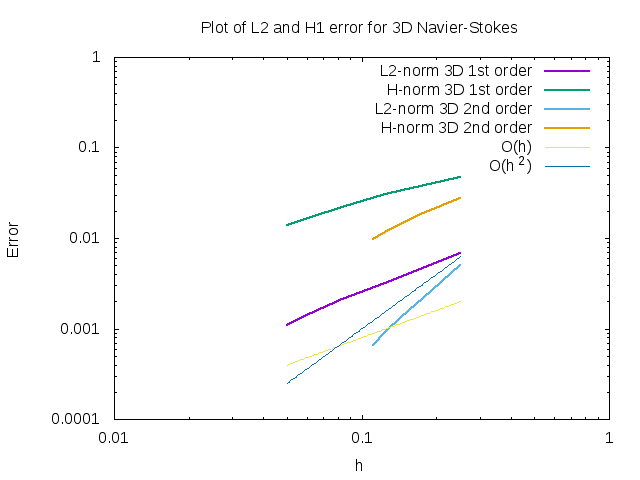
\includegraphics[width=0.7\linewidth]{NS_3D/error_NS_3D}
	\caption{}
	\label{fig:errorns3d}
\end{figure}


\newpage
Below is the FreeFEM++ code used to solve the problem above with the discritization of time using scheme $ 0 $ with convect term :
\begin{lstlisting}
load "iovtk"
load "msh3"

// Variable declaration
real nu = 1.0;
real delta=1.0;
real error,Herror;
real errormax = 0, Herrormax = 0;
real t=0;
func exactu1 = -cos(x)*sin(y)*cos(z)*exp(-2*t);
func exactu2 = sin(x)*cos(y)*cos(z)*exp(-2*t);
func exactu3 = 0.;
func dx1 = sin(x)*sin(y)*cos(z)*exp(-2*t);
func dy2 = sin(x)*(-sin(y))*cos(z)*exp(-2*t);
func dz3 = 0.;
func f1 = -cos(x)*sin(y)*cos(z)*exp(-2*t);
func f2 = sin(x)*cos(y)*cos(z)*exp(-2*t);
func f3 = (-exp(-4*t)/4)*sin(2*z)*(2*cos(2*z)+1);

int[int] rup=[0,1], rdown=[0,1], rmid=[1,1,2,1,3,1,4,1];
real zmin=0,zmax=1;

ofstream ff("1error_3D.txt");
ofstream hh("1error_H.txt");

//iteration for each mesh devider
for(int n=24; n>=4; n=n-4 )
{
real dt = 1./n; //take dt=h

// Create the mesh
mesh Th2=square(n,n);
mesh3 Th=buildlayers(Th2,n,
zbound=[zmin,zmax], labelmid=rmid, reffaceup = rup, reffacelow = rdown);
plot ( Th, ps = "NS_3D_mesh_1.ps" );

fespace Uh(Th,[P1,P1,P1,P1]);
fespace Vh(Th,P13d);
macro Grad(u) [dx(u),dy(u),dz(u)]// EOM
macro div(u1,u2,u3) (dx(u1)+dy(u2)+dz(u3)) //EOM
macro L2norm(Th,u,exactu) (int3d(Th)(square(u-exactu))) //EOM

Uh [u1,u2,u3,p];
Uh [v1,v2,v3,q];
Vh u1old, u2old, u3old;

problem navierstokes ([u1,u2,u3,p],[v1,v2,v3,q]) = 
int3d(Th) (u1*v1/dt) - int3d(Th) (convect([u1old,u2old,u3old],(-dt),u1old)*v1/dt)
+ int3d(Th) (u2*v2/dt) - int3d(Th) (convect([u1old,u2old,u3old],(-dt),u2old)*v2/dt)
+ int3d(Th) (u3*v3/dt) - int3d(Th) (convect([u1old,u2old,u3old],(-dt),u3old)*v3/dt)
+ int3d(Th,qforder=3)( Grad(u1)'*Grad(v1) +  Grad(u2)'*Grad(v2) +  Grad(u3)'*Grad(v3) //)';
- div(u1,u2,u3)*q - div(v1,v2,v3)*p)
- int3d(Th) ((f1*v1) + (f2*v2) + (f3*v3))
- int3d(Th) (delta* hTriangle * hTriangle * Grad(p)'*Grad(q))
+ on(1,u1=exactu1,u2=exactu2,u3=exactu3) ;

u1old = -cos(x)*sin(y)*cos(z) ;
u2old = sin(x)*cos(y)*cos(z) ;
u3old = 0;

for ( int it = 1; it <= n; it++ )
{
t=it*dt;
navierstokes;
error = sqrt( L2norm(Th,u1,exactu1) + L2norm(Th,u2,exactu2) + L2norm(Th,u3,exactu3));
Herror = sqrt( square(error) + L2norm(Th,dx(u1),dx1) + L2norm(Th,dy(u2),dy2) + L2norm(Th,dz(u3),dz3));
if (error > errormax) errormax = error ;
if (Herror > Herrormax) Herrormax = Herror ;
cout << "L2-error at " << t << "is " << error << "max = " << errormax << "\n" ;
cout << "H1-error at " << t << "is " << Herror << "max = " << Herrormax << "\n"; 
if(n==24){
plot ( Th, [u1,u2,u3], nbiso = 60, fill = 0, value = 1, wait = 0);
savevtk("NS_3D_1_plot"+n+"_"+it+".vtk",Th,[u1,u2,u3],p,dataname="NavSto");
plot (p, nbiso=60, fill =0, value =1, wait =0 );
}
u1old = u1; u2old=u2; u3old=u3;
}
ff << dt << "\t" << errormax << "\n" ;
hh << dt << "\t" << Herrormax << "\n" ;
cout << ">>>>>MESH>>>>> " << n << " executed \n" ;
errormax = 0;
}
//  Terminate.
//
cout << "\n";
cout << "NAVIERSTOKES:\n";
cout << "Normal end of execution.\n";
\end{lstlisting}

\newpage
We also try to use discretization of time using Adam-Bashfoth with convect term, the code is :
\begin{lstlisting}
load "iovtk"
load "msh3"

// Variable declaration
real nu = 1.0;
real delta=1.0;
real error, Herror;
real errormax = 0, Herrormax = 0;
real t=0;
func exactu1 = -cos(x)*sin(y)*cos(z)*exp(-2*t);
func exactu2 = sin(x)*cos(y)*cos(z)*exp(-2*t);
func exactu3 = 0.;
func dx1 = sin(x)*sin(y)*cos(z)*exp(-2*t);
func dy2 = sin(x)*(-sin(y))*cos(z)*exp(-2*t);
func dz3 = 0.;
func f1 = -cos(x)*sin(y)*cos(z)*exp(-2*t);
func f2 = sin(x)*cos(y)*cos(z)*exp(-2*t);
func f3 = (-exp(-4*t)/4)*sin(2*z)*(2*cos(2*z)+1);

int[int] rup=[0,1], rdown=[0,1], rmid=[1,1,2,1,3,1,4,1];
real zmin=0,zmax=1;

ofstream ff("2error_3D.txt");
ofstream hh("2error_H.txt");

//iteration for each mesh devider
for(int n=24; n>=4; n=n-4 )
{
real dt = 1./n; //take dt=h

// Create the mesh
mesh Th2=square(n,n);
mesh3 Th=buildlayers(Th2,n,
zbound=[zmin,zmax], labelmid=rmid, reffaceup = rup, reffacelow = rdown);
plot ( Th, ps = "NS_3D_mesh_2.ps" );

fespace Uh(Th,[P1,P1,P1,P1]);
fespace Vh(Th,P13d);
macro Grad(u) [dx(u),dy(u),dz(u)]// EOM
macro div(u1,u2,u3) (dx(u1)+dy(u2)+dz(u3)) //EOM
macro L2norm(Th,u,exactu) (int3d(Th)(square(u-exactu))) //EOM

Uh [u1,u2,u3,p];
Uh [v1,v2,v3,q];
Vh u1old, u2old, u3old;
Vh u1oldd, u2oldd, u3oldd;
Vh u1star,u2star,u3star;

problem navierstokesinit ([u1,u2,u3,p],[v1,v2,v3,q]) = 
int3d(Th) (u1*v1/dt) - int3d(Th) (convect([u1old,u2old,u3old],(-dt),u1old)*v1/dt)
+ int3d(Th) (u2*v2/dt) - int3d(Th) (convect([u1old,u2old,u3old],(-dt),u2old)*v2/dt)
+ int3d(Th) (u3*v3/dt) - int3d(Th) (convect([u1old,u2old,u3old],(-dt),u3old)*v3/dt)
+ int3d(Th,qforder=3)( Grad(u1)'*Grad(v1) +  Grad(u2)'*Grad(v2) +  Grad(u3)'*Grad(v3) //)';
- div(u1,u2,u3)*q - div(v1,v2,v3)*p)
- int3d(Th) ((f1*v1) + (f2*v2) + (f3*v3))
- int3d(Th) (delta* hTriangle * hTriangle * Grad(p)'*Grad(q))
+ on(1,u1=exactu1,u2=exactu2,u3=exactu3) ;

problem navierstokes ([u1,u2,u3,p],[v1,v2,v3,q]) = 
int3d(Th) (3*u1*v1/dt) - int3d(Th) (convect([u1star,u2star,u3star],(-dt),u1old)*4*v1/dt) 
+ int3d(Th) (convect([u1star,u2star,u3star],(-2*dt),u1oldd)*v1/dt)
+ int3d(Th) (3*u2*v2/dt) - int3d(Th) (convect([u1star,u2star,u3star],(-dt),u2old)*4*v2/dt) 
+ int3d(Th) (convect([u1star,u2star,u3star],(-2*dt),u2oldd)*v2/dt)
+ int3d(Th) (3*u3*v3/dt) - int3d(Th) (convect([u1star,u2star,u3star],(-dt),u3old)*4*v3/dt) 
+ int3d(Th) (convect([u1star,u2star,u3star],(-2*dt),u3oldd)*v3/dt)
+ int3d(Th,qforder=3)( Grad(u1)'*Grad(v1) +  Grad(u2)'*Grad(v2) +  Grad(u3)'*Grad(v3) //)';
- div(u1,u2,u3)*q - div(v1,v2,v3)*p)
- int3d(Th) ((f1*v1) + (f2*v2) + (f3*v3))
- int3d(Th) (delta* hTriangle * hTriangle * Grad(p)'*Grad(q))
+ on(1,u1=exactu1,u2=exactu2,u3=exactu3) ;

u1old = -cos(x)*sin(y)*cos(z) ;
u2old = sin(x)*cos(y)*cos(z) ;
u3old = 0;

for ( int it = 1; it <= n; it++ )
{
t=it*dt;
if (it==1) {navierstokesinit;}
else {
navierstokes;
error = sqrt( L2norm(Th,u1,exactu1) + L2norm(Th,u2,exactu2) + L2norm(Th,u3,exactu3));
Herror = sqrt( square(error) + L2norm(Th,dx(u1),dx1) + L2norm(Th,dy(u2),dy2) + L2norm(Th,dz(u3),dz3));
if (error > errormax) errormax = error ;
if (Herror > Herrormax) Herrormax = Herror ;
cout << "L2-error at " << t << "is " << error << "max = " << errormax << "\n" ;
cout << "H1-error at " << t << "is " << Herror << "max = " << Herrormax << "\n"; 
}
if(n==24){
plot ( Th, [u1,u2,u3], nbiso = 60, fill = 0, value = 1, wait = 0);
savevtk("NS_3D_2_plot"+n+"_"+it+".vtk",Th,[u1,u2,u3],p,dataname="NavSto");
plot (p, nbiso=60, fill =0, value =1, wait =0 );
}
u1oldd = u1old; u2oldd = u2old; u3oldd = u3old; 
u1old = u1; u2old=u2; u3old=u3;
u1star = 2*u1old-u1oldd; u2star = 2*u2old-u2oldd; u3star = 2*u3old-u3oldd;
}
ff << dt << "\t" << errormax << "\n" ;
hh << dt << "\t" << Herrormax << "\n" ;
cout << ">>>>>MESH>>>>> " << n << " executed \n" ;
errormax = 0;
}
//  Terminate.
//
cout << "\n";
cout << "NAVIERSTOKES:\n";
cout << "Normal end of execution.\n";
\end{lstlisting}

%We also try other exact solution
%\begin{eqnarray}\nonumber
%u &=& (u_{1},u_{2},u_{3}) \\ \nonumber
%u_{1} &=& \sin(x)\cos(y)\cos(z)\cos(2\pi t)\\ \nonumber
%u_{2} &=& \cos(x)\sin(y)\cos(z)\cos(2\pi t)\\ \nonumber
%u_{3} &=& -2\cos(x)\cos(y)\sin(z)\cos(2\pi t)\\ \nonumber
%p&=& \sin(x)\sin(y)\sin(z)\cos(2\pi t)
%\end{eqnarray}
%such that equation (\ref{Navier-Stokes}) is satisfied with $ f = (f_{1},f_{2},f_3) $, where
%\begin{eqnarray} \nonumber
%f_{1} &=& \sin(x)\cos(y)\cos(z)(3\cos(2\pi t)-2\pi\sin(2\pi t)) + \sin(x)\cos(x)(\cos(2\pi t))^2((\cos(y)\cos(z))^2 \\ \nonumber & &-(\sin(y)\cos(z))^2+2(\cos(y)\sin(z))^2) + \cos(x)\sin(y)\cos(z)\cos(2\pi t) \\ \nonumber
%f_{2} &=& \cos(x)\sin(y)\cos(z)(3\cos(2\pi t)-2\pi \sin(2\pi t)) + \sin(y)\cos(y)(\cos(2\pi t))^2((\cos(x)\cos(z))^2 \\ \nonumber & &-(\sin(x)\cos(z))^2+2(\cos(x)\sin(z))^2) + \sin(x)\cos(y)\sin(z)\cos(2\pi t); \\ \nonumber
%f_{3} &=& 2\cos(x)\cos(y)\sin(z)(2\pi\sin(2\pi t)-3\cos(2\pi t)) + 2\sin(z)\cos(z)(\cos(2\pi t))^2((\sin(x)\cos(y))^2\\ \nonumber & &+(\cos(x)\sin(y))^2+2(\cos(x)\cos(y))^2) + \sin(x)\sin(y)\cos(z)\cos(2\pi t);
%\end{eqnarray}

\end{document}